\section{Results}
\label{results}
The results are included for the Topic Modelling experiments and the Stock Modelling experiments. 

\subsection{Topic Modelling}
For the topic modelling, the results are included for both LDA examples, the initial example on one day's worth of GDELT events data and the USA/China March-April data. The results also include the TF-IDF top values for the USA/China data, and the K Means results on the same dataset.

\subsubsection{Initial LDA}
The LDA models are included for running on the one day event data and the USA/China dataset. 
%\paragraph{Initial LDA}
Initially a topic model was run on one day's worth of Event data. The day was the 1st of November 2019. This was done as a reference point before running the LDA models on the specific USA/China chosen data.

There were two different topic models tried. Firstly one model with 3 topics was tried and then one model with 5 topics. It was unknown how many topics would be present in the data, thus two different values were chosen, one with a smaller number of topics (3), and a slightly larger number of topics (5). The two values were tested to see if a smaller or a larger number of topics would represent any topics present in the data. The top words from each model are shown in word cloud format in Figures \ref{fig:single3wc} and \ref{fig:single5wc}. Alongside the word cloud, for each topics, the weight and the word count of the top words was also calculated and plotted. 
	
\begin{figure}[H]
	\centering
	\subfloat[Word Cloud 3 Topics]{  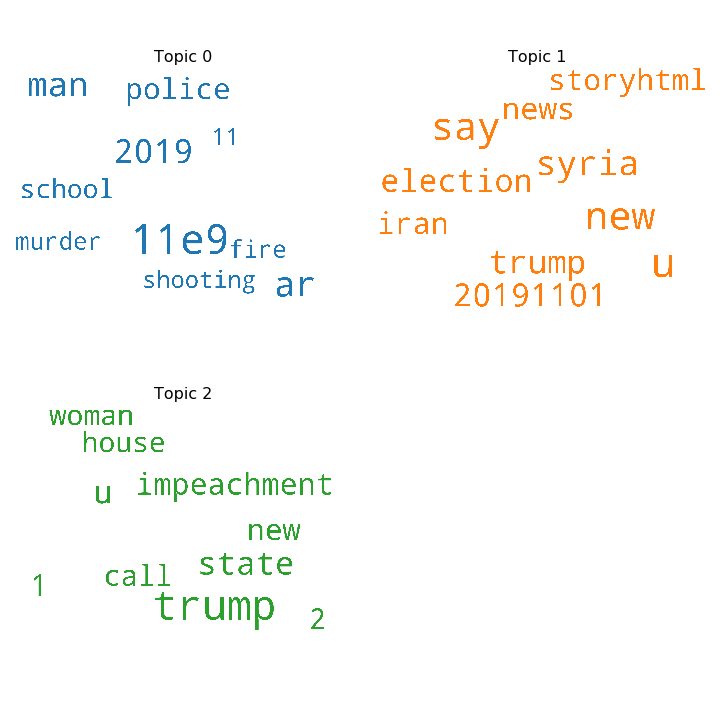
\includegraphics[width=0.8\textwidth]{images/single/word_cloud_single_3_topics.png}\label{fig:single3wc}}\\
	\subfloat[Word Weights 3 topics]{  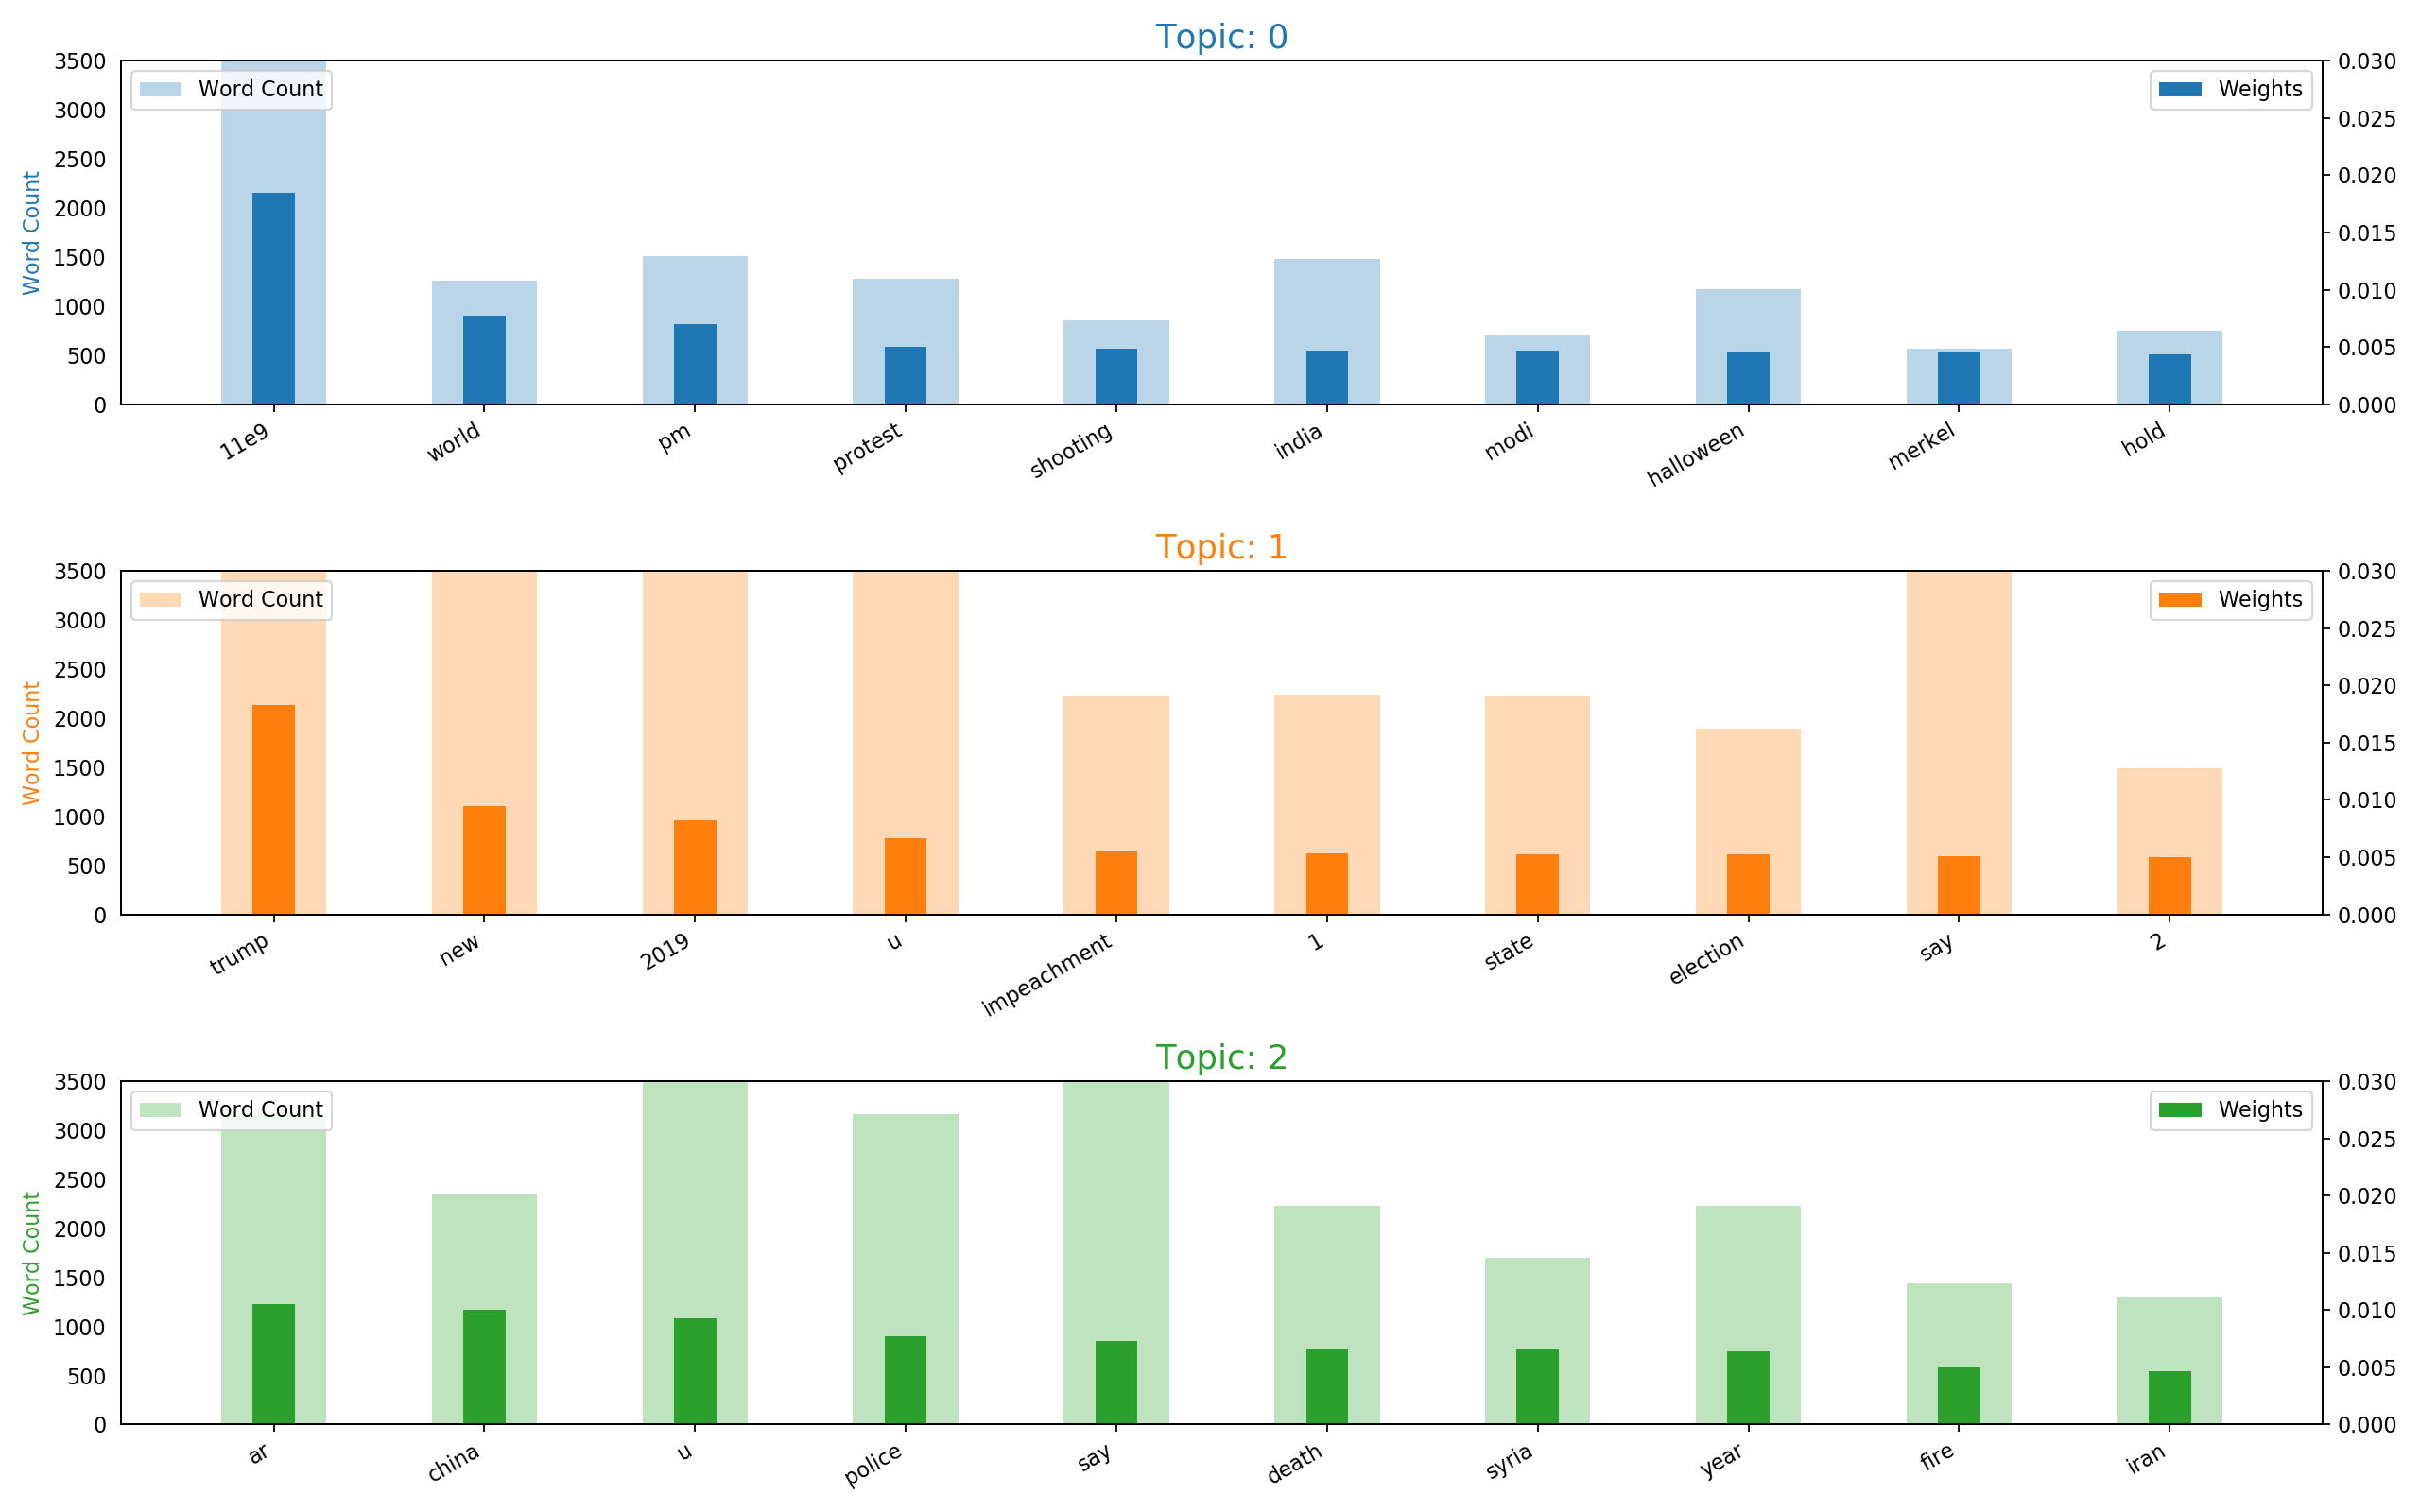
\includegraphics[width=0.8\textwidth]{images/single/word_weights_single_3_topics.png}\label{fig:single3ww}}\\
	
	\caption{Single Day Word Clouds and Word Weights for 3 topics}
	\label{fig:single3}
\end{figure}

Examining the word clouds for the model with three topics, there are not any clear topics which are apparent. Topic 2 could vaguely be about the impeachment process for Donald Trump, Topic 0 appears to be focused on police brutality as a topic, and Topic 1 could broadly be referred to in terms of international news. Examining the word importances, the main theme across topics is that the word count is not the same as the word importance, in that some words have much higher occurrences, but lower weights and vice versa. This is perhaps to be expected, as the word count and importance do not have to be linked.

\begin{figure}[H]
	\centering
	\subfloat[Word Cloud 5 Topics]{  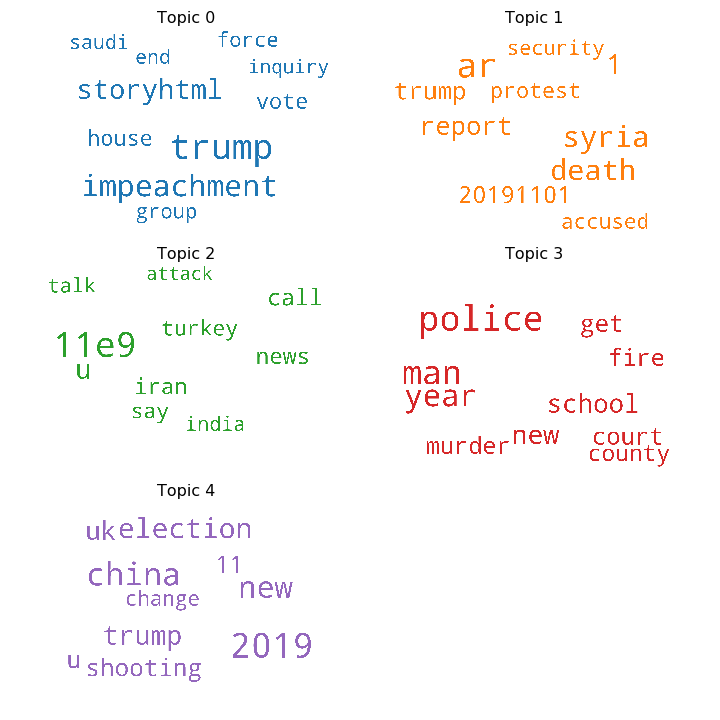
\includegraphics[width=0.8\textwidth]{images/single/word_cloud_single_5_topics.png}\label{fig:single5wc}}\\
	\subfloat[Word Weights 5 topics]{  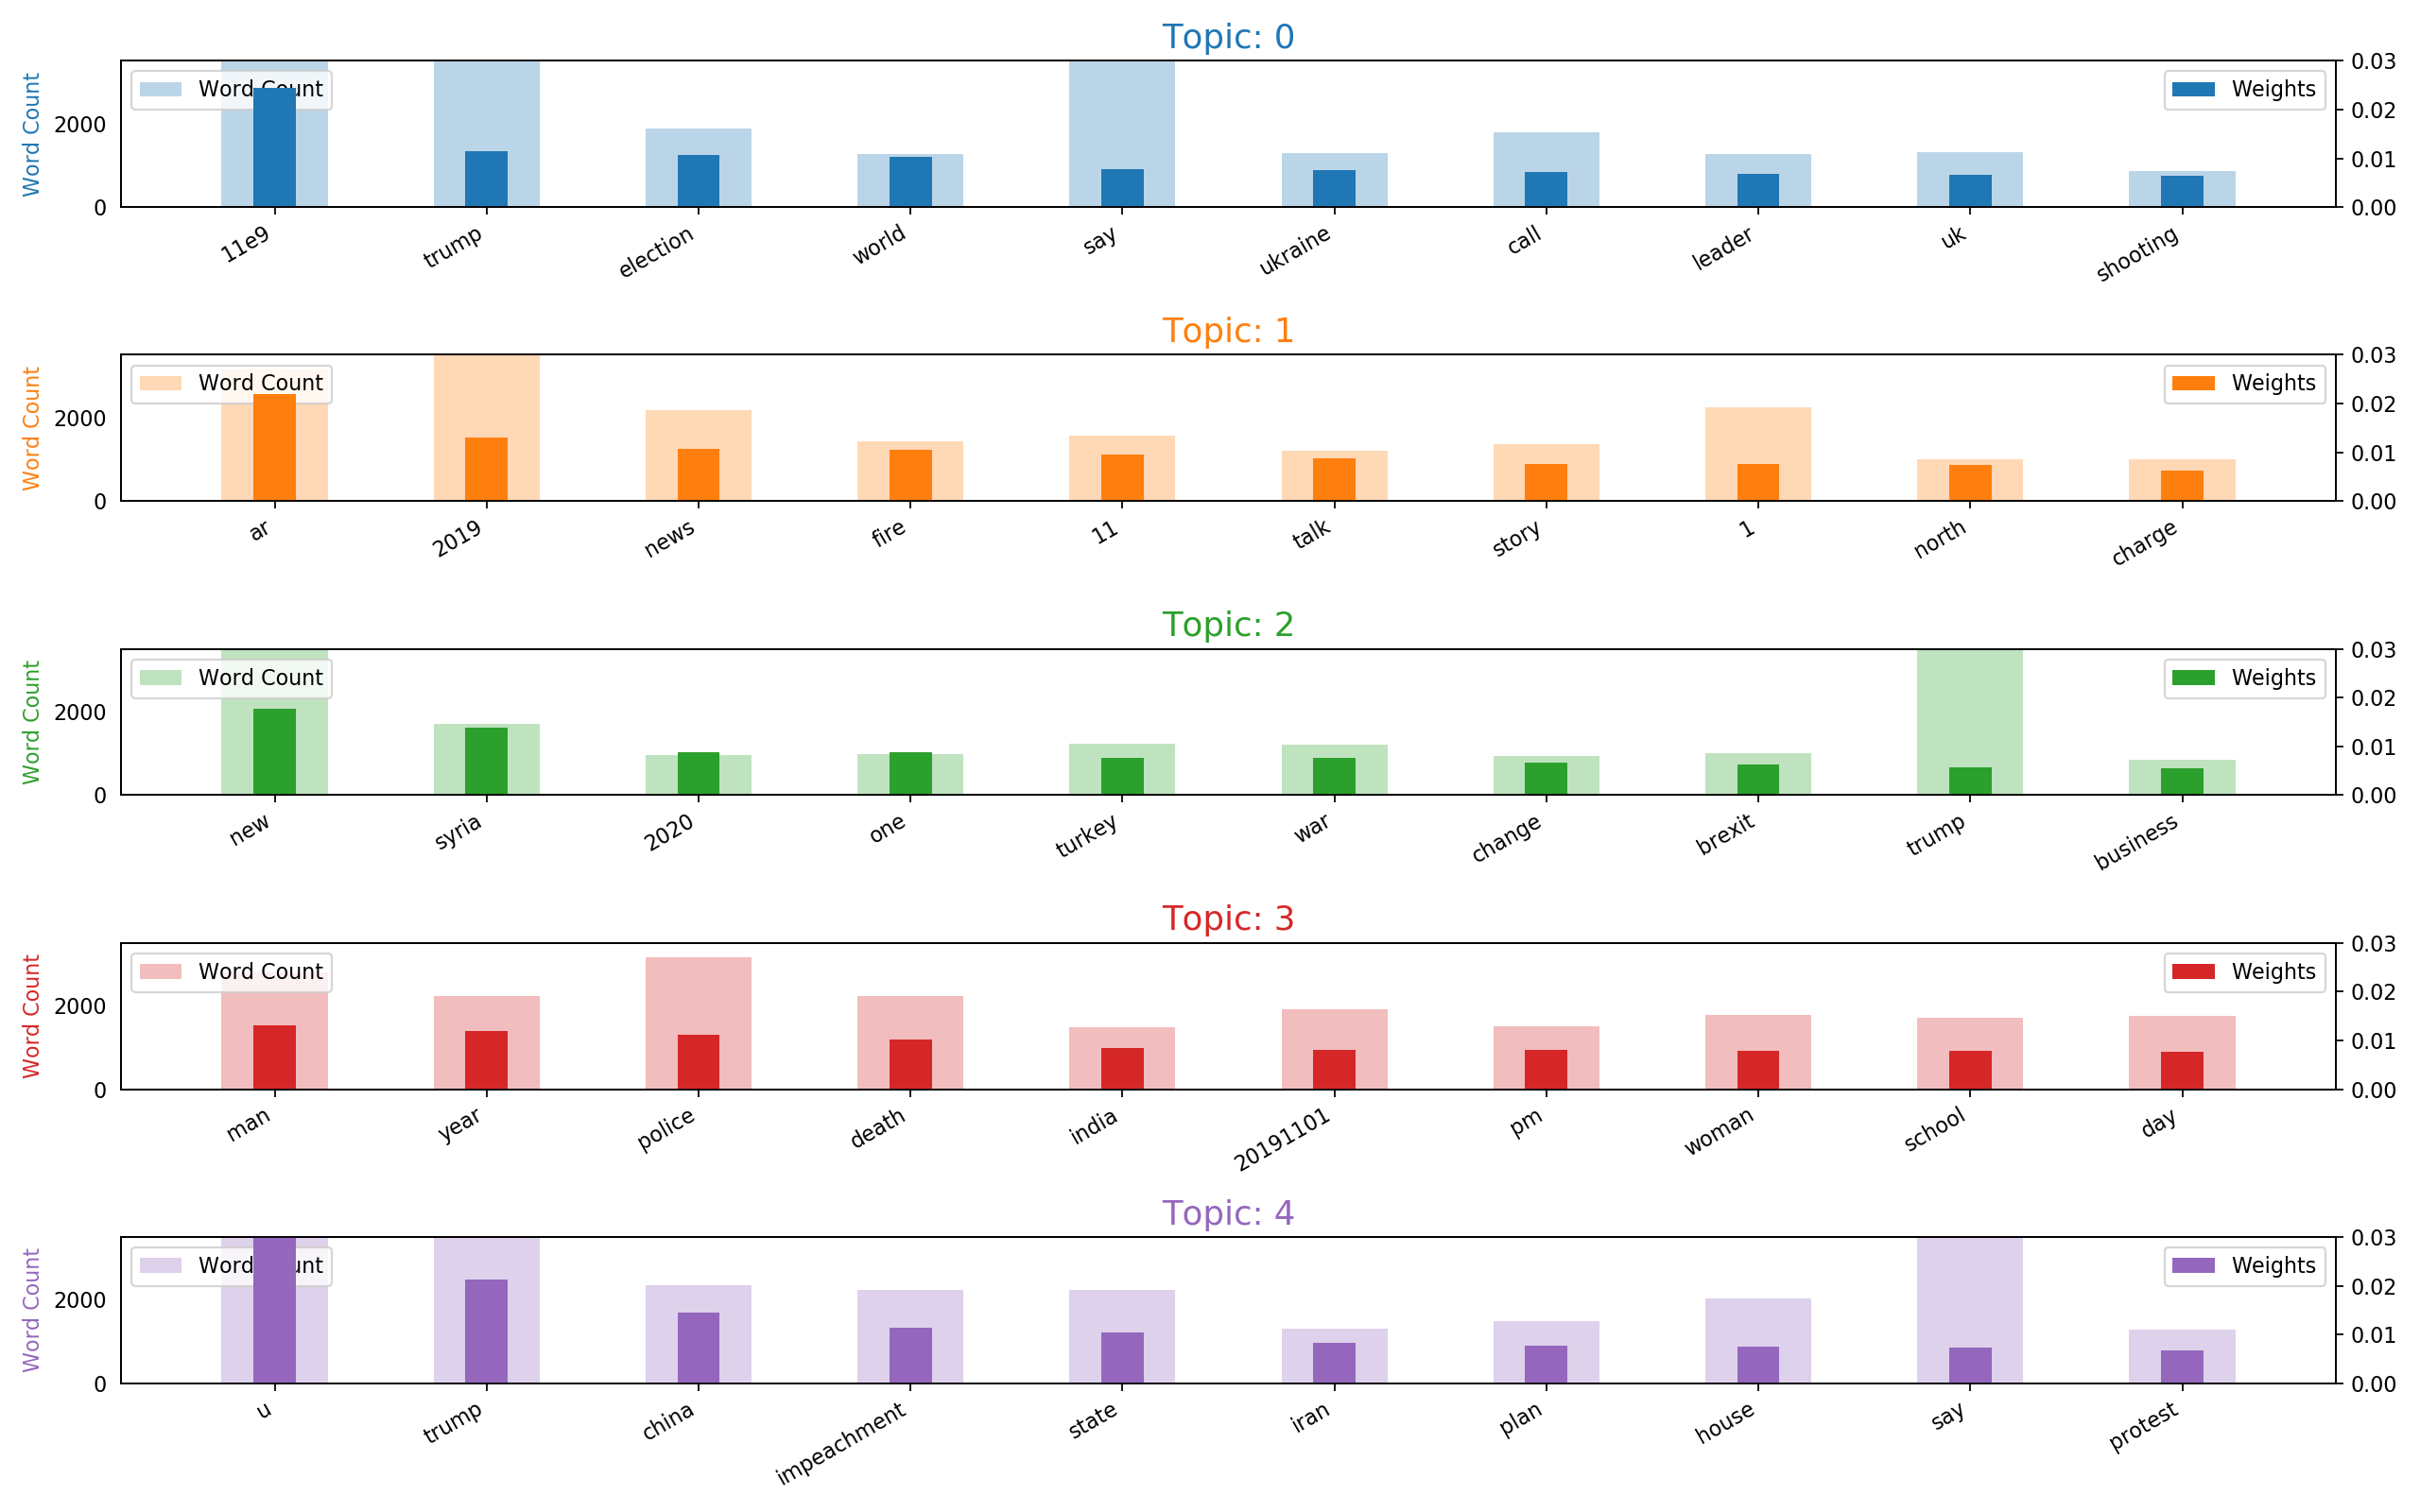
\includegraphics[width=1\textwidth]{images/single/word_weights_single_5_topics.png}\label{fig:single5ww}}\\
	
	\caption{Single Day Word Clouds and Word Weights for 5 topics}
	\label{fig:single5}
\end{figure}	

Examining the 5 topic model, the topics are much closer together, its very difficult to find a central topic for each topic, Topic 3 could potentially be about police and court information, but aside from that there does not appear to any coherency otherwise, with words like Trump being in multiple topics and international countries spread across topics. The word importance and weight plot also does not reveal anything new, like the previous model, the word's count is not related to the importance and perhaps expectedly, the words in the topics are not related to each other.

\subsubsection{USA/China Data}
A similar procedure was used for the USA/China data, but models with 2, 3, and 4 topics each were tried, as it was not completely clear from the initial LDA model whether a smaller or larger amount of topics would represent the data better. The word clouds of the results and the subsequent word importances to each topic are shown in Figures \ref{fig:usa2}, \ref{fig:usa3}, and \ref{fig:usa4}. 
\begin{figure}[H]
	\centering
	\subfloat[USA/China Word Cloud 2 Topics]{  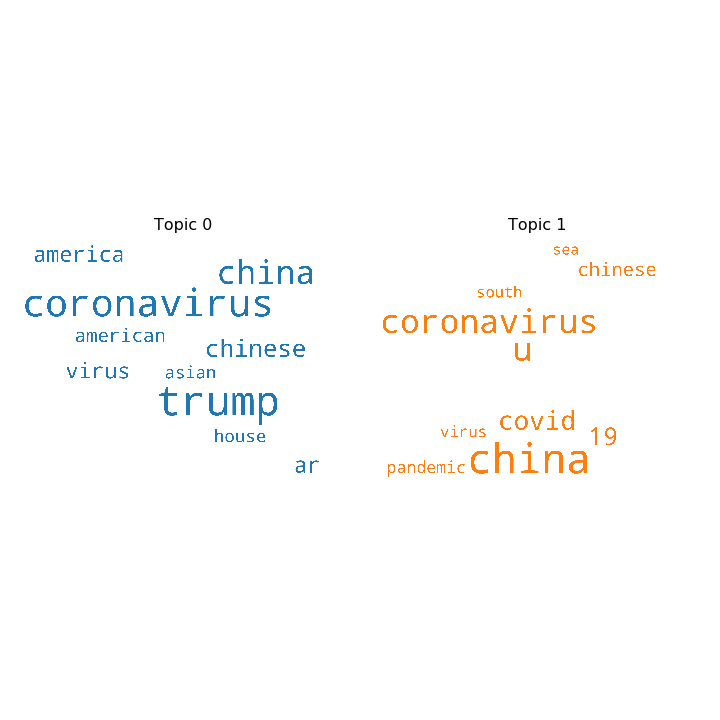
\includegraphics[width=0.6\textwidth]{images/uschina/word_cloud_usa_2_topics.png}\label{fig:us2wc}}\\
	\subfloat[USA/China Word Weights 2 topics]{  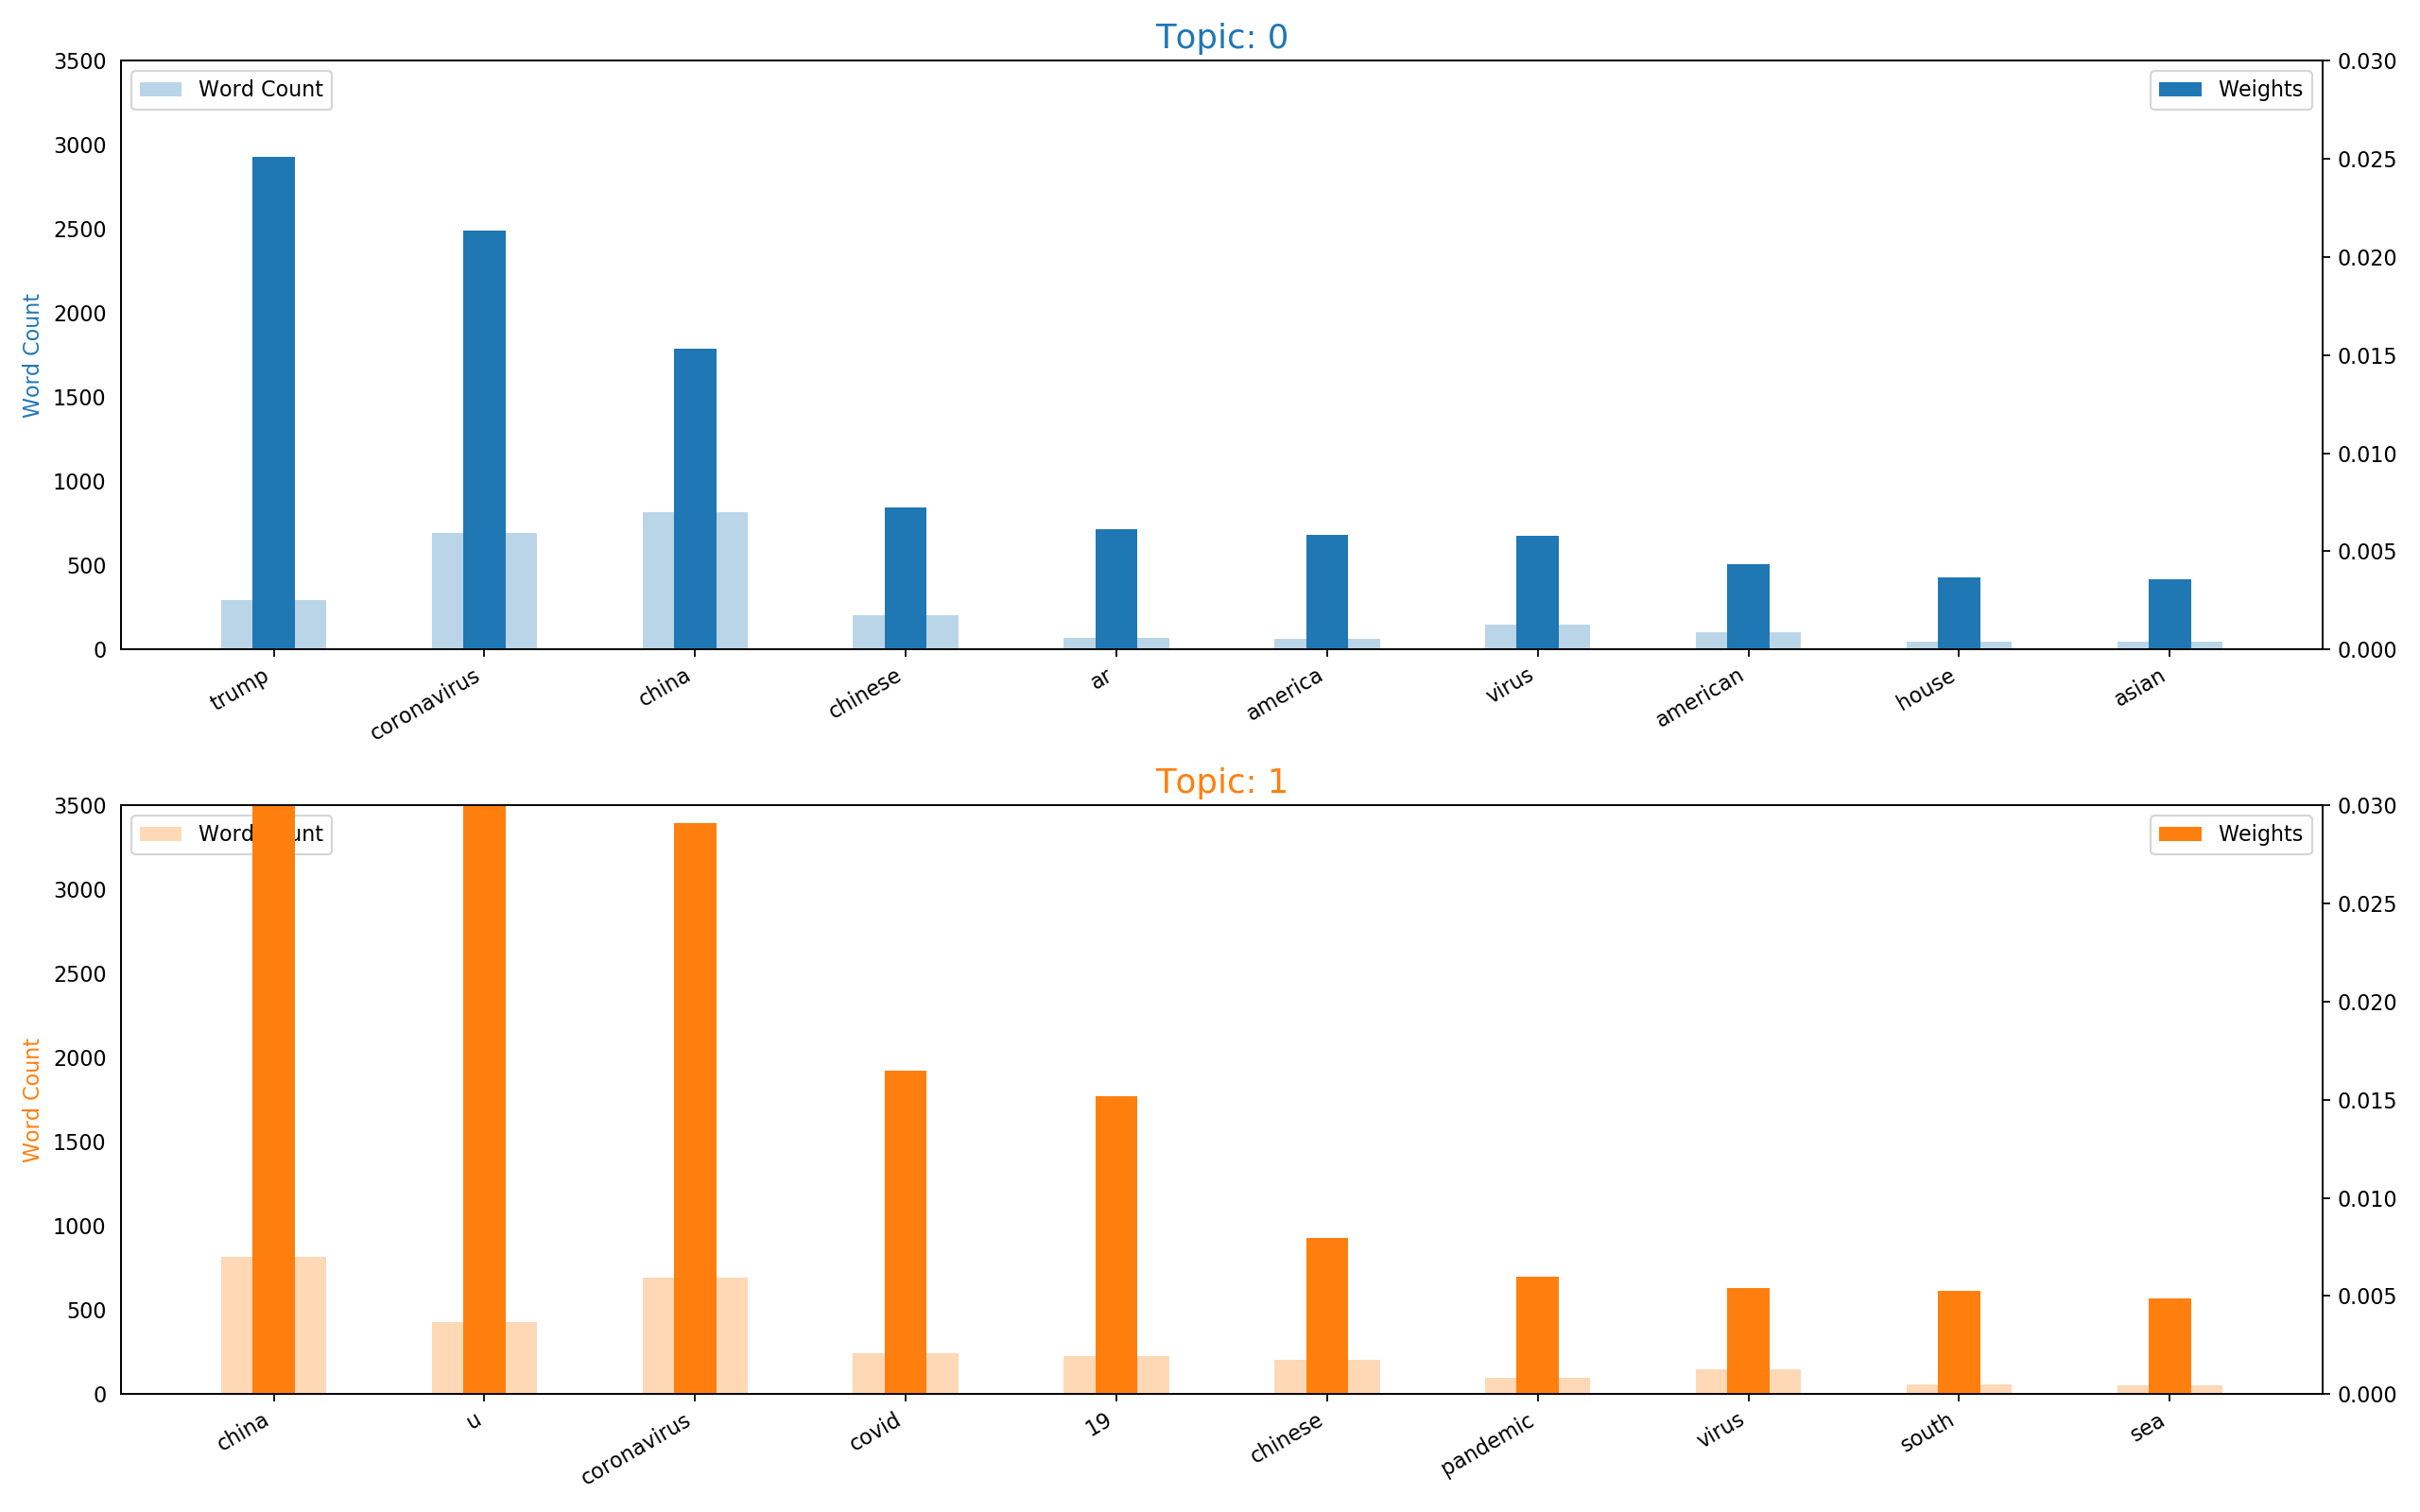
\includegraphics[width=0.8\textwidth]{images/uschina/word_weights_usa_2_topics.png}\label{fig:us2ww}}\\
	
	\caption{USA/China Word Clouds for 2 topics}
	\label{fig:usa2}
\end{figure}
Examining the first LDA model which had 2 topics on the USA China data, the themes are very similar. Words related to the pandemic, and words such as China and Trump appear in both topics, which suggest the model has not been effective in differentiating between the topics effectively. Looking at the word weights in Figure \ref{fig:us2ww}, for all of the words, the weights are all higher than the word counts. The highest word weights by topic are Trump, Coronavirus, China for Topic 0 and China, Coronavirus, and `U` for Topic 1 . `U` appears appears to be another issue with the parsing.  
\begin{figure}[H]
	\centering
	\subfloat[USA/China Word Cloud 3 Topics]{  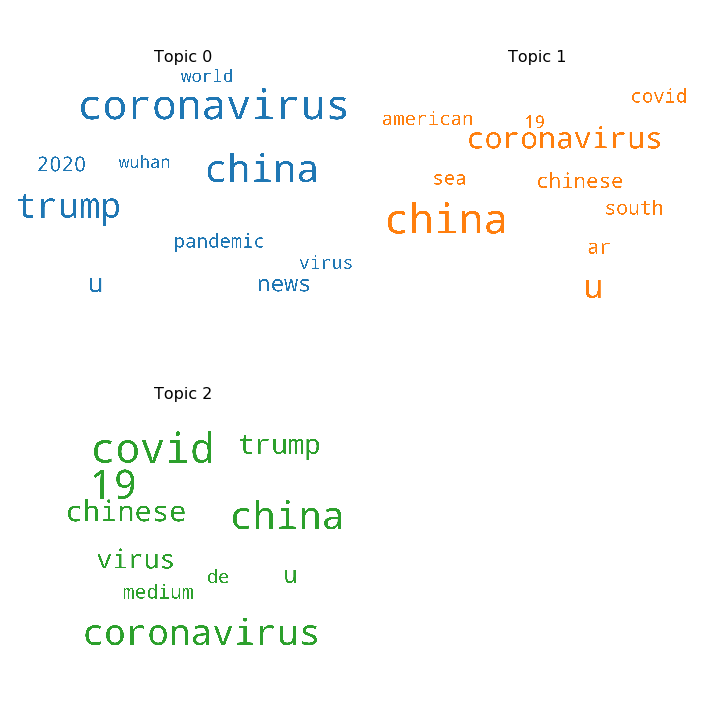
\includegraphics[width=0.6\textwidth]{images/uschina/word_cloud_usa_3_topics.png}\label{fig:us3wc}}\\
	\subfloat[USA/China Word Weights 3 topics]{  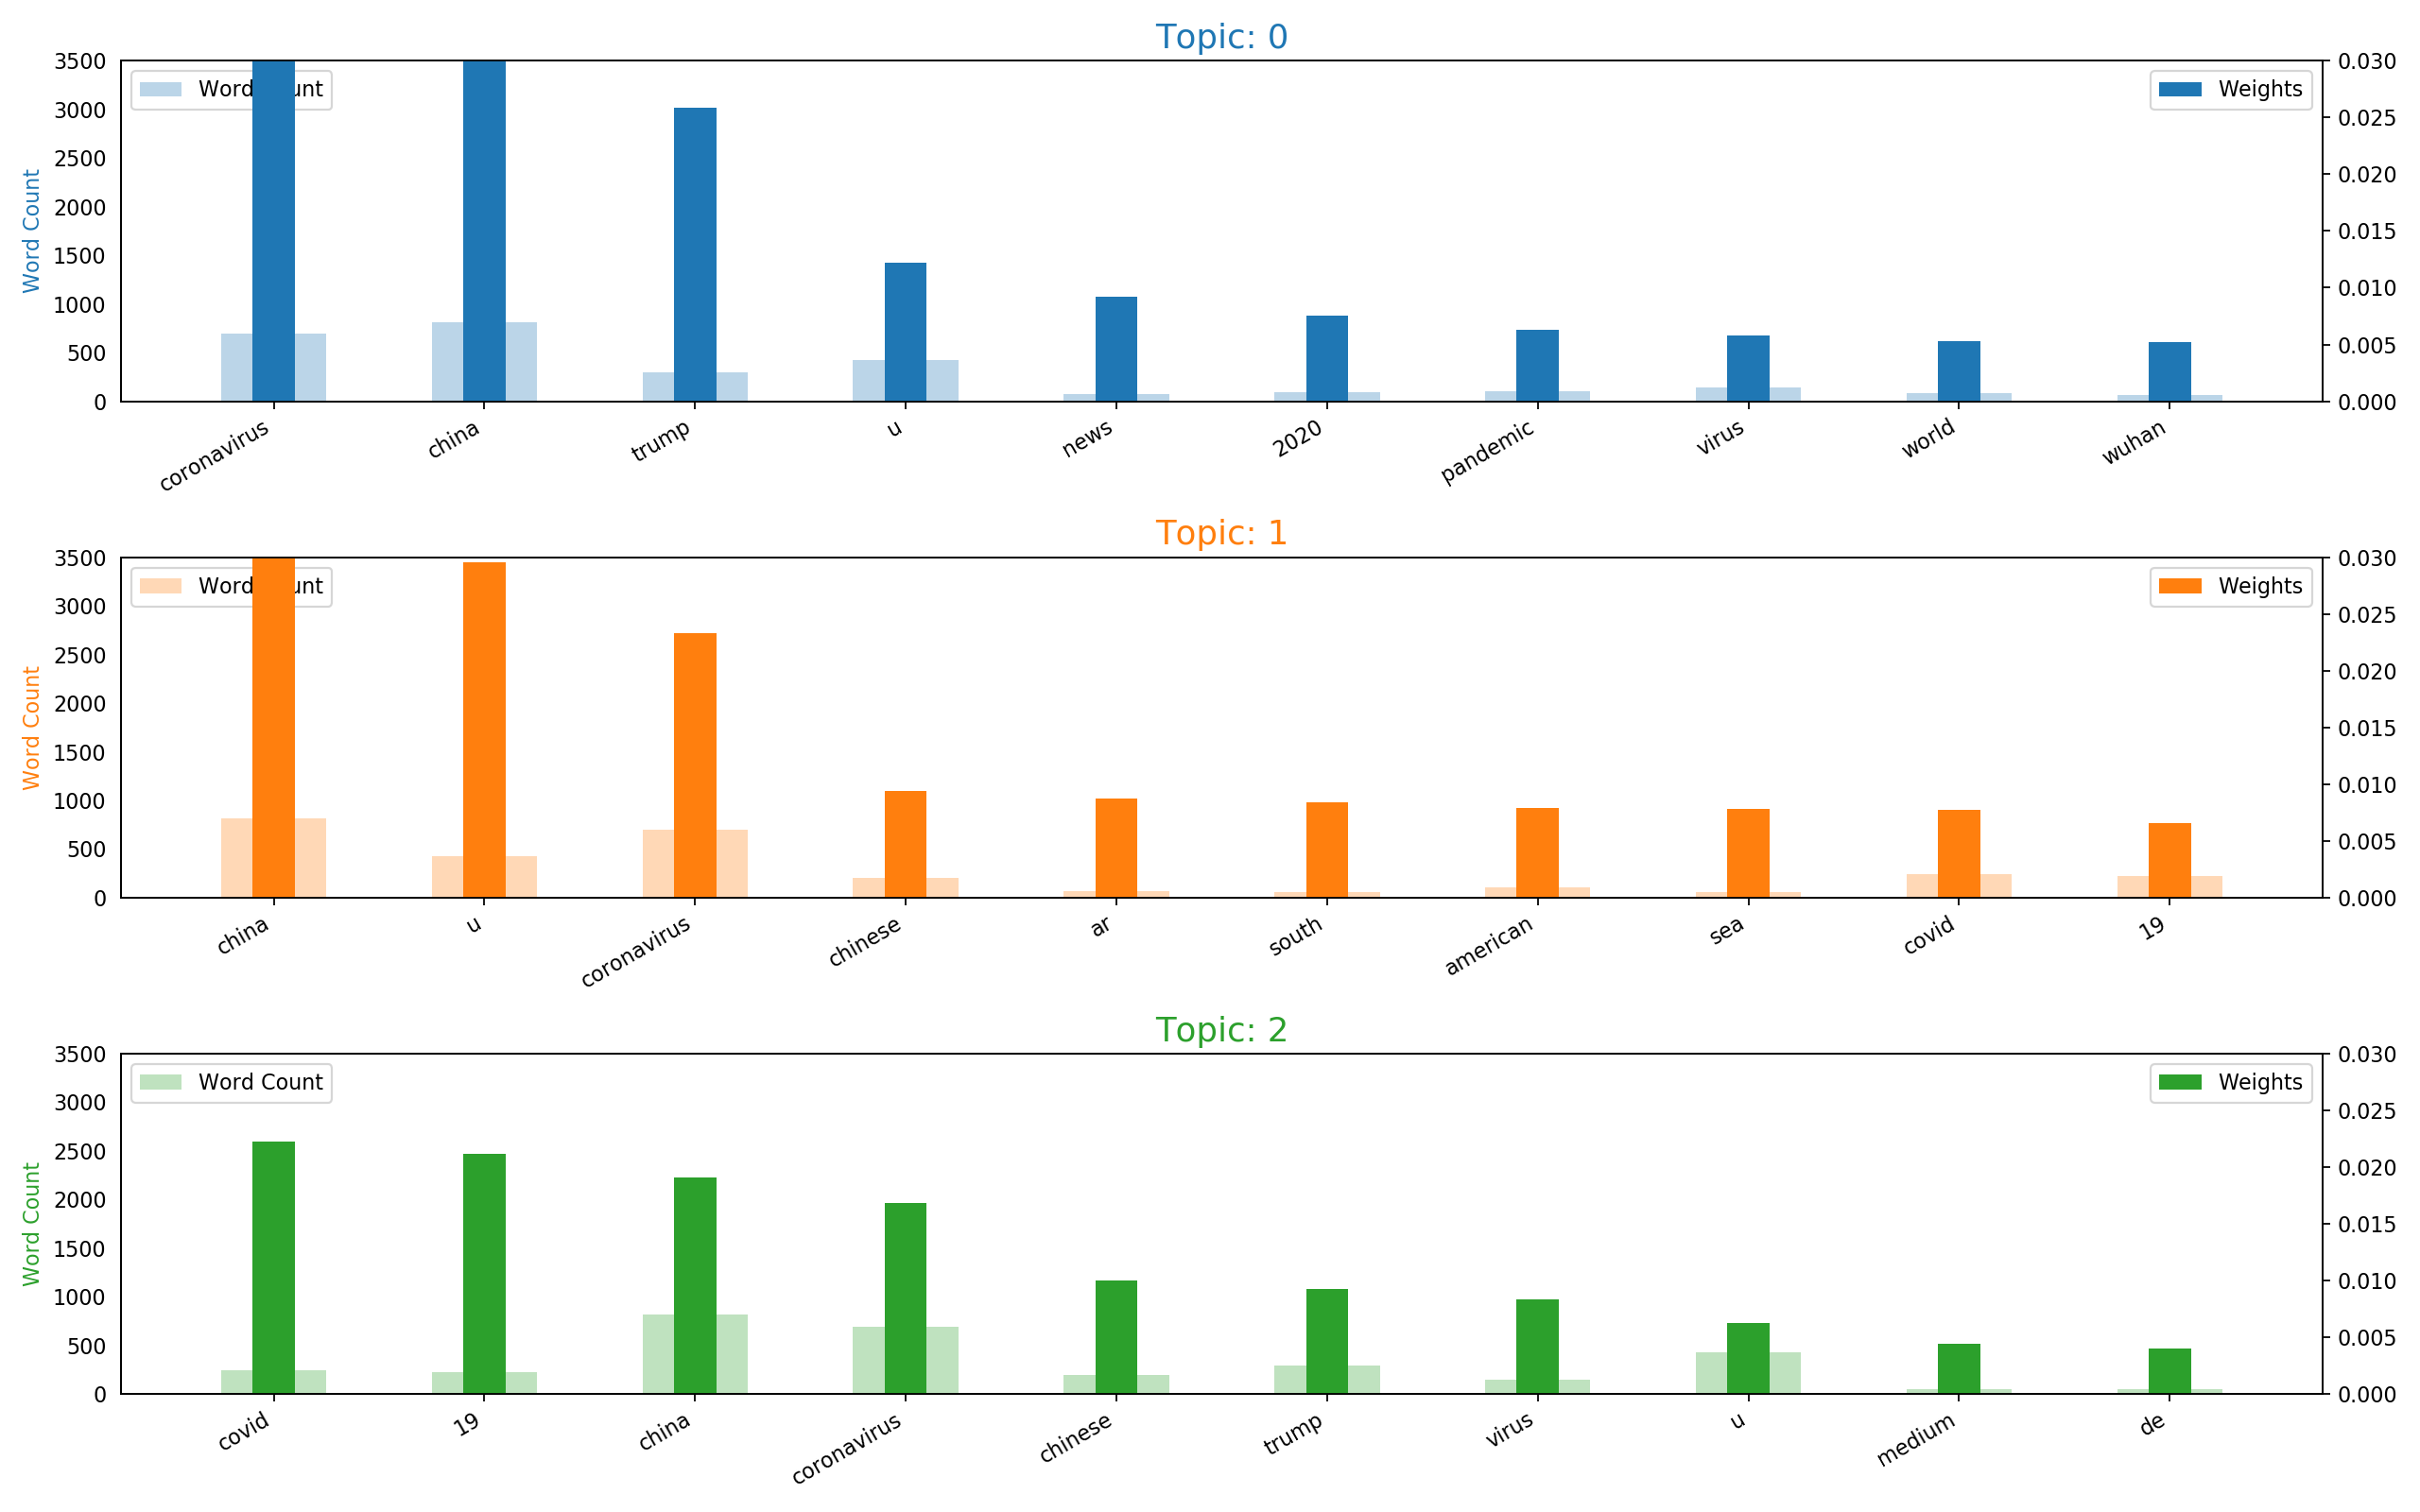
\includegraphics[width=0.8\textwidth]{images/uschina/word_weights_usa_3_topics.png}\label{fig:us3ww}}\\
	
	\caption{USA/China Word Clouds for 3 topics}
	\label{fig:usa3}
\end{figure}

Looking the the three topic model, the topics are even closer together than the two topic model. The main words as before appear in all of the topics, suggesting the topic model hasn't separated any topics well. The word weights are also similar to the two topic model. One of the differences between the two topic and the three topic model is the 3rd topic weights are noticeably smaller than the first and second topics. 

\begin{figure}[H]
	\centering
	\subfloat[USA/China Word Cloud 4 Topics]{  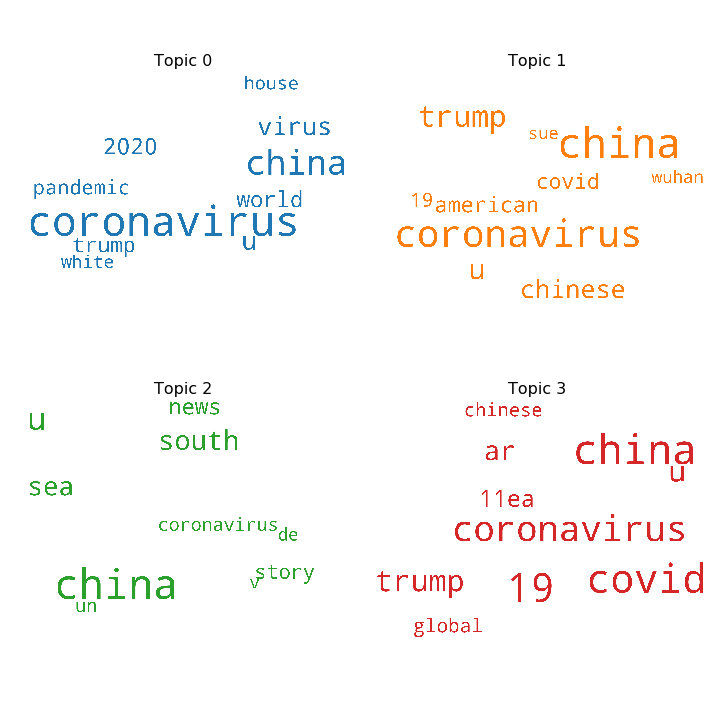
\includegraphics[width=0.6\textwidth]{images/uschina/word_cloud_usa_4_topics.png}\label{fig:us4wc}}\\
	\subfloat[USA/China Word Weights 4 topics]{  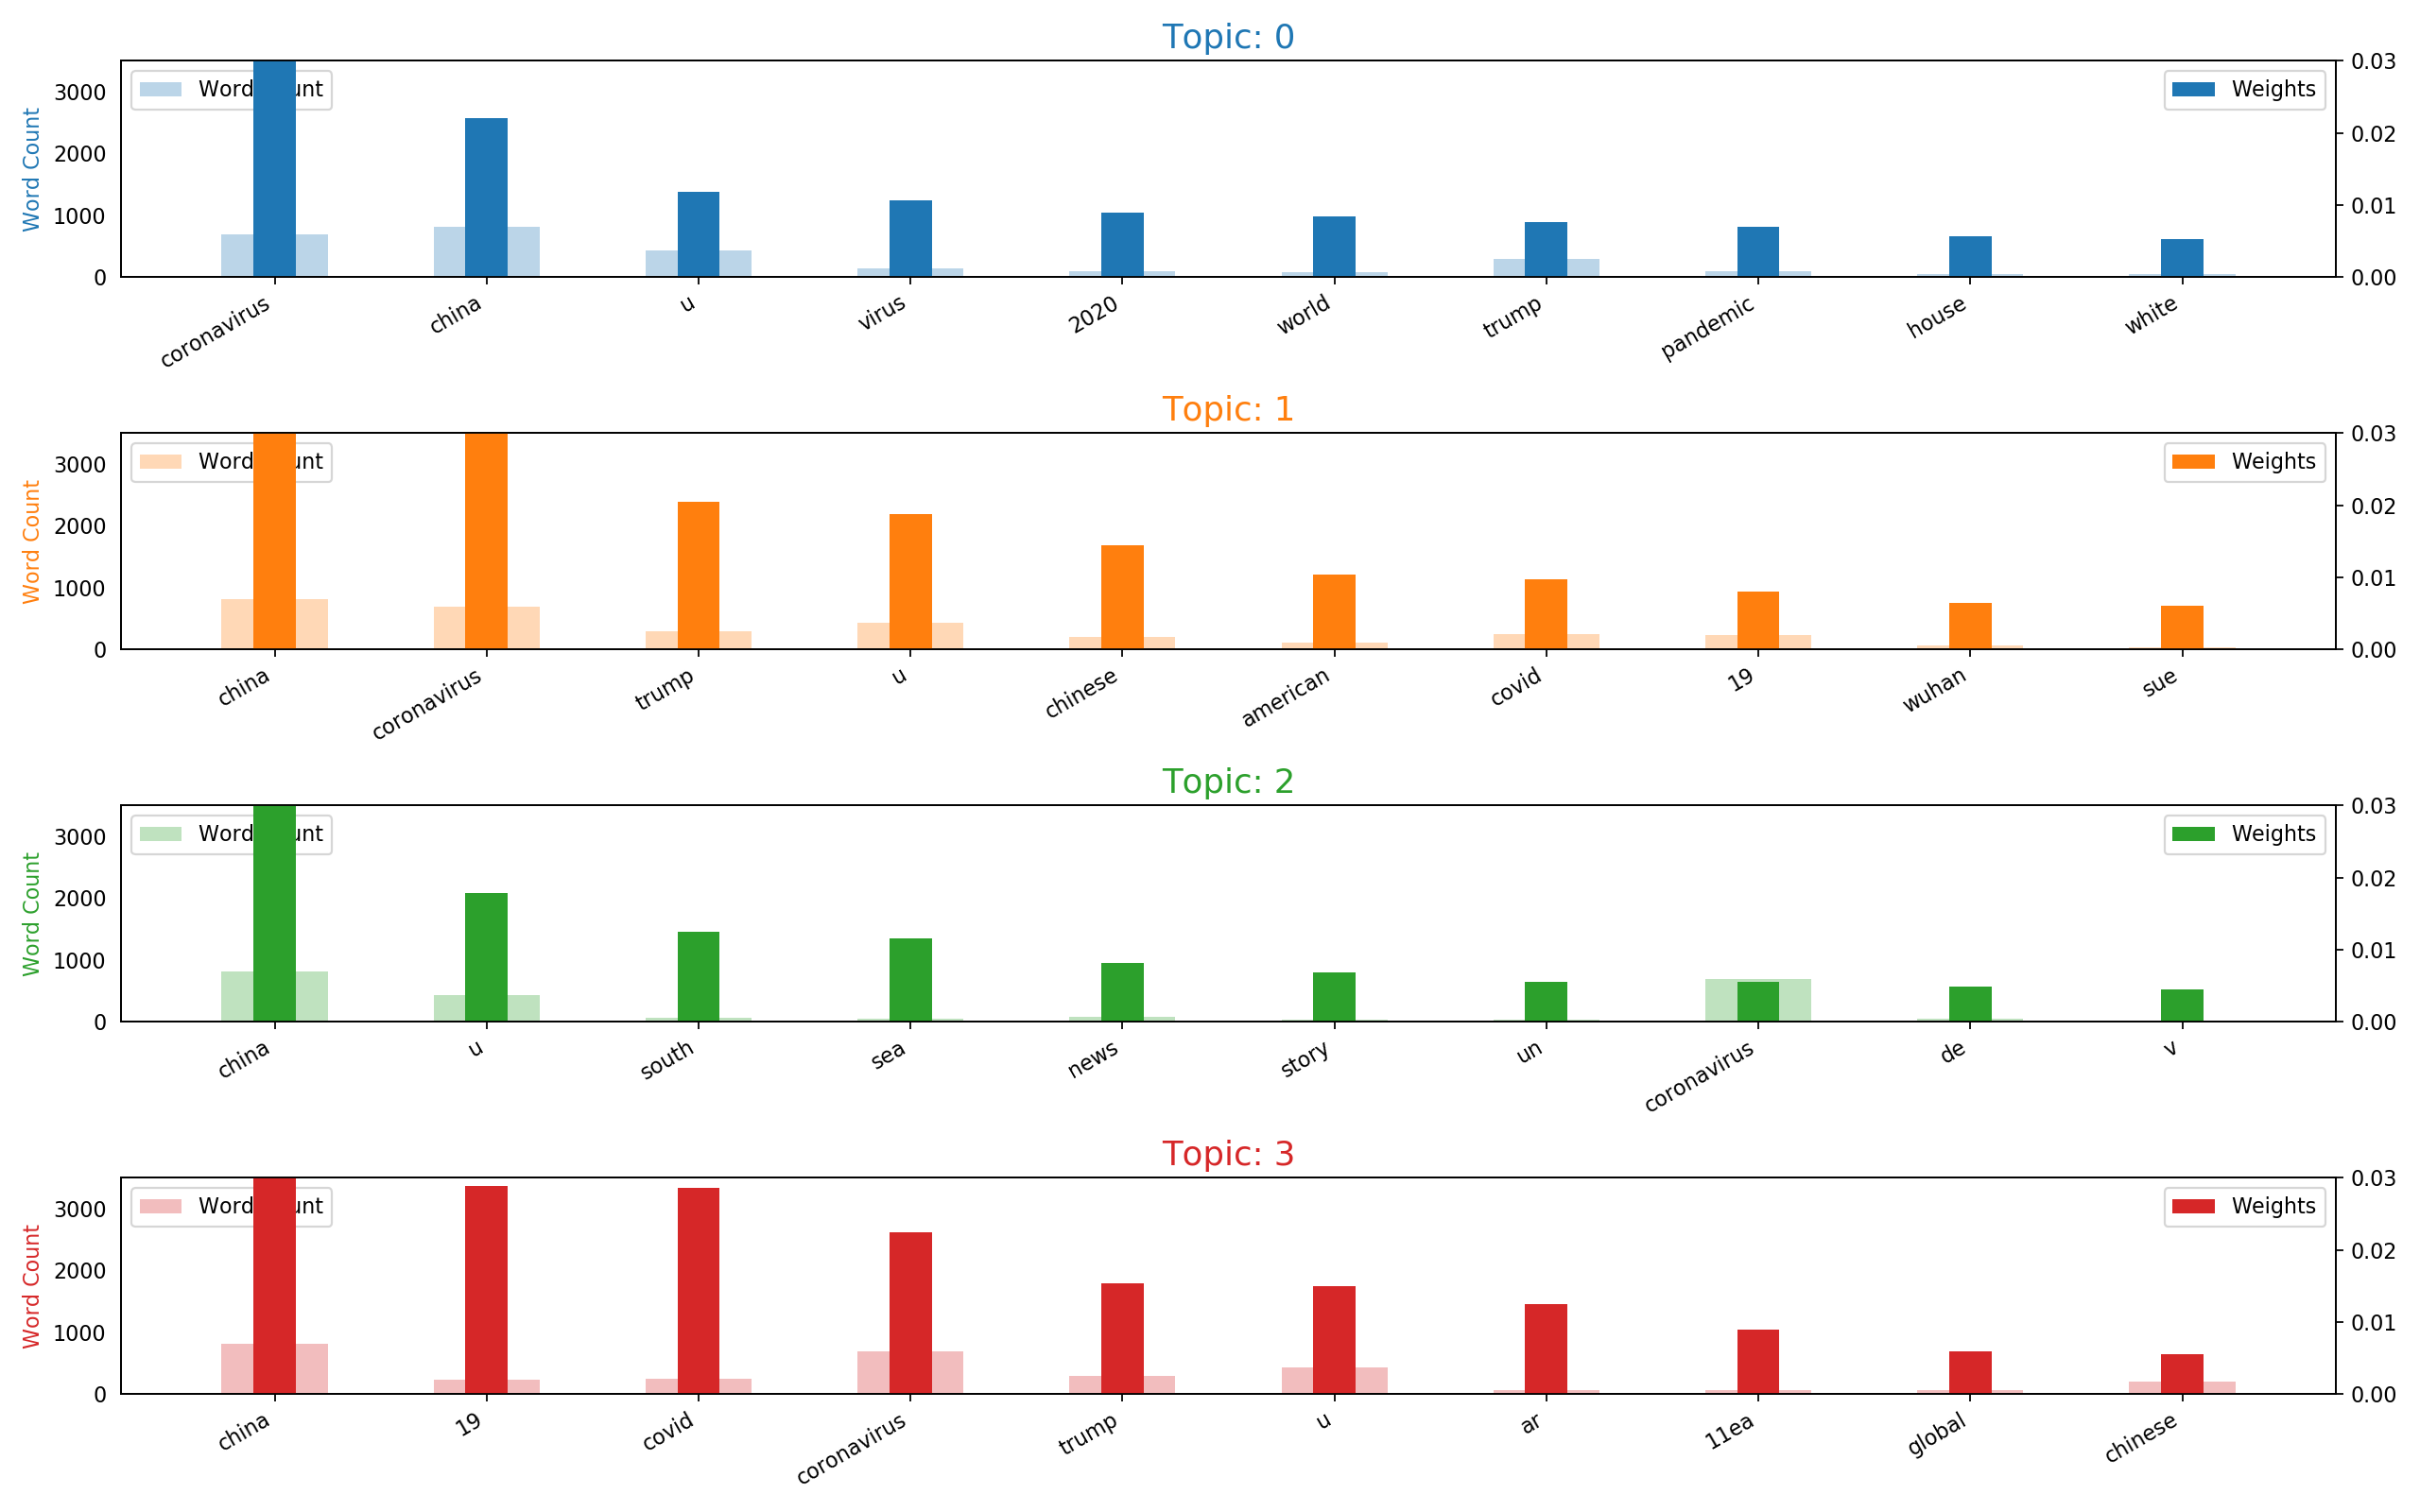
\includegraphics[width=0.8\textwidth]{images/uschina/word_weights_usa_4_topics.png}\label{fig:us4ww}}\\
	
	\caption{USA/China Word Clouds for 4 topics}
	\label{fig:usa4}
\end{figure}

The 4 topic model behaves in a similar manner to the previous 2 topic models. the main words are split across the 4 topics with no real distinction between the topics present. 
\subsubsection{TF-IDF}
The top TF-IDF terms are shown for the USA China data across the corpus in Figure \ref{fig:tfidfusachina}. This data was achieved by taking the average of the TF-IDF values across the entire dataset. The average values are slightly lower across the corpus compared to individual documents, as there will be a number of documents where specific words have TF-IDF values of 0, as those words do not exist in those documents. These 0 TF-IDF values are included in the mean calculations as the parsing process for URLs is not perfect in retrieving headlines. If the 0 TF-IDF values were excluded from the averaging calculations, the top words by TF-IDF would be non-representative of the whole corpus. This is due to some `words` present only in a small number of documents, e.g. `words` which represent parsing errors. These words have high TF-IDF values in the documents they exist in. Thus if their 0 TF-IDF values from all other documents are not included in the averaging calculation, these words would have artificially high TF-IDF values across all of the documents and not be representative of the actual top words in the corpus.

\begin{figure}[H]
	\centering
	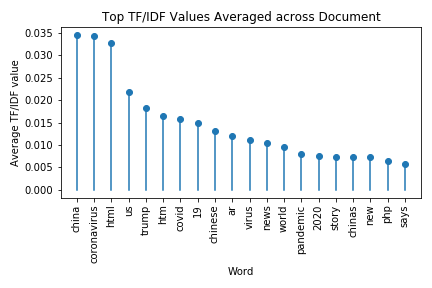
\includegraphics[width=0.8\textwidth]{Images/usa_stem_tfidf.png}
	\caption{Plot of the top 15 words which used TF-IDF in the USA/China specific data}
	\label{fig:tfidfusachina}
\end{figure}

Perhaps as expected, the most important and often occurring words are China and coronavirus.  Amongst the top words are also US, and Trump, along with variations of China and covid-19 and references to the pandemic. This is most interesting as a result, as something which no one had heard of prior to January/February dominated the news in March and April.

One of the other main words which pops up is html. This is most likely as a result of the fact that most of the URLs end with `.htm` or `.html`, and during the parsing html gets treated as a commonly occurring word. It was not removed as there could be legitimate stories which have the word in them. 

For the top values, the distribution of the tf-idf values across documents was calculated, excluding the 0 values. This is shown in Figure \ref{fig:tfidfdist}. The distributions are different to each other, but both follow a similar pattern in having a centre of the distribution be around a Tf-IDF value of around 0.25. One of the notable exceptions to this is the word `ar`, which is another error as a result of parsing. World and news both have a spike later on, but that is most likely due to the smaller sample size.

\begin{figure}[H]
	\centering
	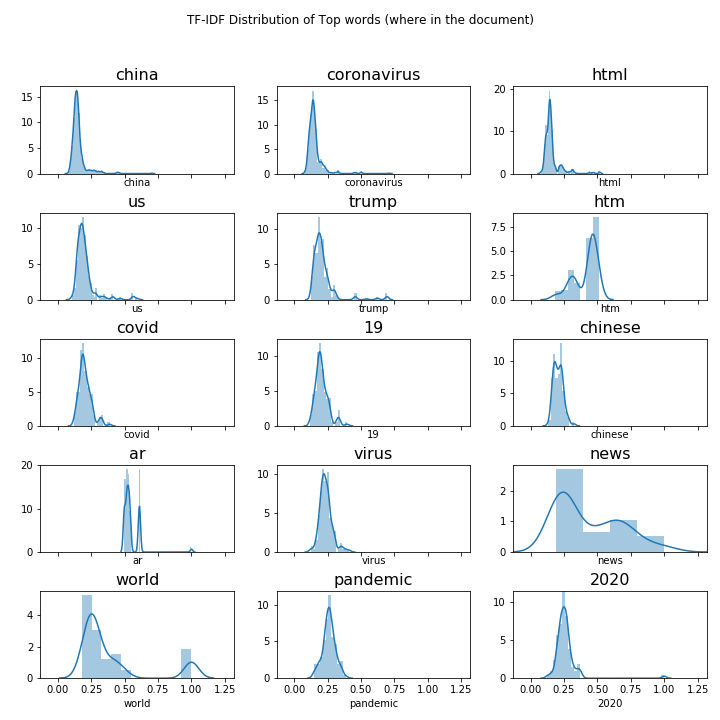
\includegraphics[width=0.8\textwidth]{Images/usa_tfidf_top_distribution.png}
	\caption{Distribution of the TF-IDF values across documents of the top 15 words (excluding documents where the Tf-IDF value was 0)}
	\label{fig:tfidfdist}
\end{figure}

\subsubsection{K Means}
Similar to the LDA models, the K-means was tried with 2, 3, and 4 clusters. A range of cluster numbers were tried, as after running the initial LDA, and the USA/China LDA models, it was not evidently clear which `K` would be most appropriate. The word cloud of the top words are shown in Figures \ref{fig:wck2}, \ref{fig:wck3}, and \ref{fig:wck4}. Alongside the word clouds, the clusters were decomposed into 2 and 3 dimensions by both Principal Component Analysis (PCA) and T-distributed Stochastic Neighbour Embedding (T-SNE) \cite{maaten2008visualizing}. This was to see whether the clusters had been successful in separating the data at any level. This is shown for the different number of cluster in Figures \ref{fig:k2pca}, \ref{fig:k3pca}, and \ref{fig:k4pca} respectively. Furthermore, the Mahalanobis and Euclidean distances were plotted for all of the points associated with a cluster for all of the clusters present. This is shown in Figures \ref{fig:distk2}, \ref{fig:distk3}, and \ref{fig:distk4} respectively. 

To compare the efficacy of clusters in being able to filter information, the Mahalanobis distance from centre of clusters for variety of phrases was calculated, and plotted in Figures \ref{fig:wordsk2}, \ref{fig:wordsk3}, and \ref{fig:wordsk4}, alongside the distribution of points for each cluster. For all of the Mahalanobis distances, the phrases were several orders of magnitude out from the distribution of points for each cluster, so the Mahalanobis distance results were logged before being plotted.  
\paragraph{Clustering with k=2}
\begin{figure}[H]
	\centering
	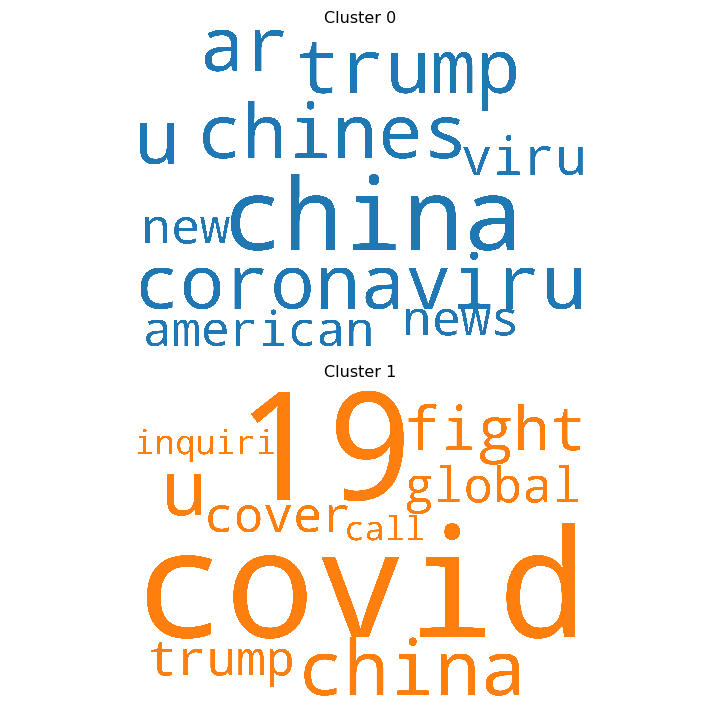
\includegraphics[width=0.8\textwidth]{images/kmeans_word_cloud_k=2.png}
	\caption{Word Cloud for k=2 clusters}
	\label{fig:wck2}
\end{figure}
Examining the word cloud created for a two cluster model, a similar picture appears as with the LDA models. There are several words which are close to both of the clusters, which, in a similar fashion to the LDA model, mean that any topics present are not being differentiated. This is evident in Figure \ref{fig:k2pca}, in which both T-SNE and PCA in both 2 and 3 dimensions show that the clusters are not distinct from each other. Interestingly, both the 2d and 3D PCA plots, Figures \ref{fig:pca2k2} and \ref{fig:pca3k2}, appear to show defined boundaries between clusters, however, the cluster definitions aren't what a human would draw. The main caveat with the PCA and T-SNE plots is that the proportion of explained variance in the dimensions selected is extremely poor, for both the 2 dimensional and 3 dimensional decomposition, each dimension captures less than 0.01 of the explained variance. This means that the clusters may still be accurately portraying the data in another dimension/combination of dimensions, but it is not visible in this dimension. 

\begin{figure}[H]
	\centering
	\subfloat[2D PCA k=2]{  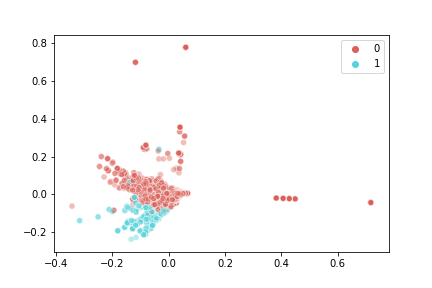
\includegraphics[width=0.45\textwidth]{images/kmeans_2d_pca_k=2.png}\label{fig:pca2k2}}
	\subfloat[3D PCA k=2]{  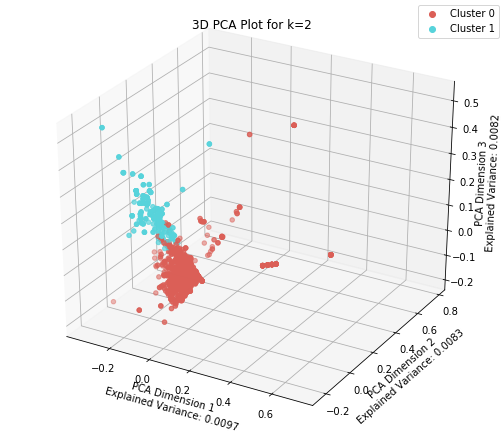
\includegraphics[width=0.45\textwidth]{images/kmeans_3d_pca_k=2.png}\label{fig:pca3k2}}\\
	\subfloat[2D T-SNE k=2]{  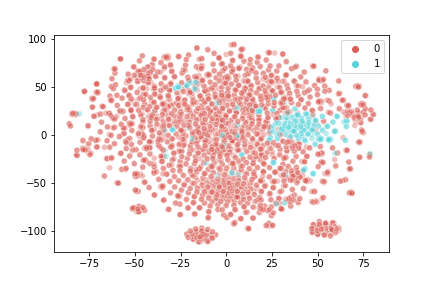
\includegraphics[width=0.45\textwidth]{images/kmeans_2d_tsne_k=2.png}\label{fig:ts2k2}}
	\subfloat[3D T-SNE k=2]{  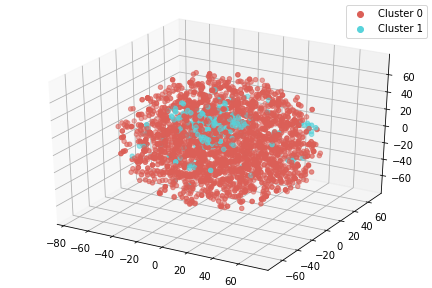
\includegraphics[width=0.45\textwidth]{images/kmeans_3d_tsne_k=2.png}\label{fig:ts3k2}}\\
	\caption{Decompositions of the clusters in 2 and 3 dimensions using PCA and T-SNE for k=2}
	\label{fig:k2pca}
\end{figure}
Examining the Mahalanobis distances for the two clusters, there does not appear to be any noticeable pattern, the distributions are slightly bimodal, compared to the Euclidean distances, which appears to be slightly normally distributed shape wise, though normality would not be expected as the 0 distance would be the cluster centre, from which the distances are measured. The majority of points are associated with cluster 0, with the rest going to Cluster 1.
\begin{figure}[H]
	\centering
	\subfloat[Mahalanobis Distance]{  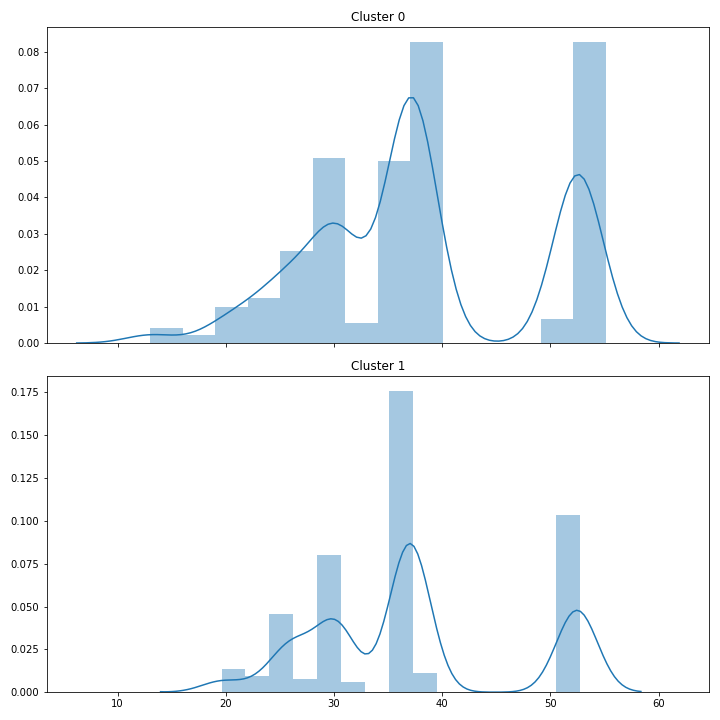
\includegraphics[width=0.45\textwidth]{images/kmeans_mahalanobis_distance_k=2.png}\label{fig:mhk2}}
	\subfloat[Euclidean Distances]{  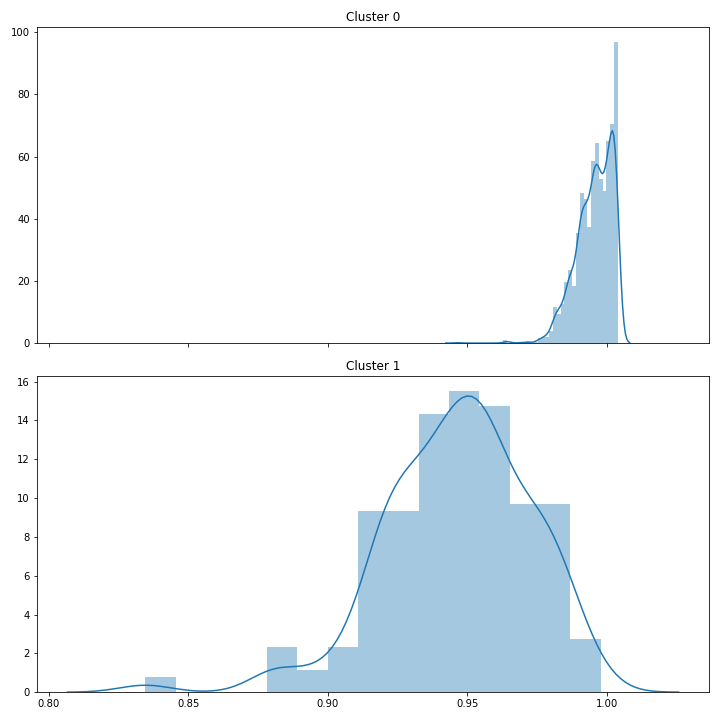
\includegraphics[width=0.45\textwidth]{images/kmeans_euclidean_distance_k=2.png}\label{fig:euk2}}\\
	
	\caption{Cluster Distances (Mahalanobis and Euclidean) for k=2 clusters}
	\label{fig:distk2}
\end{figure}

Comparing the results plotted on the log scale shown in Figure \ref{fig:wordsk2}, the first thing which becomes apparent is that the distances for the words appears to be the same between clusters, i.e. all phrases tested are equally far from both cluster 0 and cluster 1, this is perhaps unsurprising as the distance from both clusters is extremely large. Comparing the words themselves, aside from the individual word `covid`, the phrases are fairly close together, with what appears to be two sets of lines. The first lines are the `coronavirus hits remote utah`, and the `aboriginal peoples australia complain` with the remainder of the headlines making up the remainder of the lines, nearly all of the results are between 27 and 28 in terms of the absolute logged Mahalanobis distance. 
\begin{figure}[H]
	\centering
	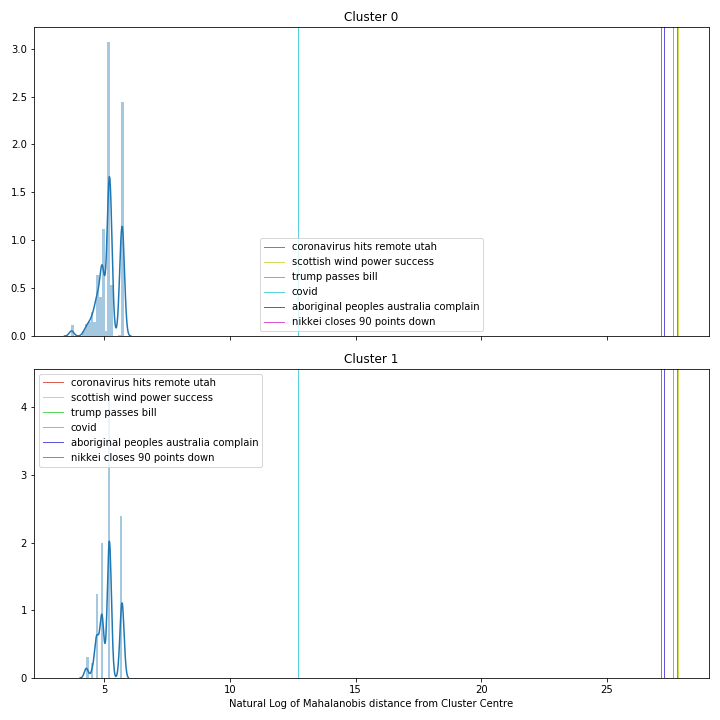
\includegraphics[width=0.8\textwidth]{images/words_kmeans_mahalanobis_distance_k=2.png}
	\caption{Log of Mahalanobis Distances for Clusters and Selected Phrases for k=2 clusters}
	\label{fig:wordsk2}
\end{figure}

\paragraph{Clustering when k=3 or k=4} 
When the number of clusters was increased to 3 or 4, it was found that there was no material change in either the topic word clouds or the decomposition plots. Thus, the word cloud, decomposition plots, and Mahalanobis distance plots are included in the appendices \ref{k3} and \ref{k4}. The word clouds for both k=3 and k=4 behaved the same as k=2, where the topics were all very similar, and the decomposition plots suggest the cluster definitions are definitively useful, and the boundaries are not as clear as they were for k=2.  There are a few features of note however. For each cluster model tried, there were 2 sets of points away from the main cluster, but when examined, these represented the points associated with the parsing errors from the URLs. The cluster Mahalanobis distances appear to be bimodal with the same range of distances for the points. As expected, the Mahalanobis distance for the selected phrases were similar distances away, with the pattern of distances being similar.

\subsection{Modelling Stock Prices}
The table of prediction accuracies for the different models is shown in Table \ref{table:modaccuracy}. This is the percentage of days over the prediction interval of May and June that each model was able to predict correctly. Several models had similar accuracy scores, though it should be noted that the predictions were on a very small dataset, so even one or two correct incorrect predictions could sway the result considerably. 

The manually lagged models appeared to be the least best, in these models 5 days worth of previous days were added as 5 features to the data, and no other averaging methodology applied. The Random Forests classifiers appeared to do well with whatever data structure was used. Furthermore, models which applied moving window calculations did well, with on average the exponentially smoothed models doing the best.

With all of that taken into consideration, the best model was picked on the basis of being exponential and the random forests. Exponential was chosen as all of the models with exponential smoothing generally did better than other types of data smoothing. Similarly, the Random Forests was good across the board, thus the best model picked was one a Random Forests model which performed exponential smoothing.
\begin{table}[H]
	\centering 
\begin{tabular}{lr}

	Classifier &  Accuracy \\
	\hline
	Reference Classifier with Previous Day & 0.750\\
	\hline
                                  Naive Bayes &     0.750 \\
Logistic Regression &     0.750 \\
Averaged Random Forests &     0.750 \\
Gaussian Averaged Random Forests &     0.750 \\
Exponential Naive Bayes &     0.750 \\
Exponential Logistic Regression &     0.750 \\
Exponential Random Forests &     0.750 \\
Random Forests &     0.625 \\
Support Vector Machine &     0.625 \\
Averaged Naive Bayes &     0.625 \\
Averaged Logistic Regression &     0.625 \\
Averaged Support Vector Machine &     0.625 \\
Gaussian Averaged Naive Bayes &     0.625 \\
Gaussian Averaged Logistic Regression &     0.625 \\
Gaussian Averaged Support Vector Machine &     0.625 \\
Exponential Support Vector Machine &     0.625 \\
Manually 4 day lagged Random Forests &     0.625 \\
Neural Network & 0.500 \\
Manually 4 day lagged Naive Bayes &     0.500 \\
Manually 4 day lagged Logistic Regression &     0.500 \\
Manually 4 day lagged Support Vector Machine &     0.375 \\
	

\end{tabular}

	\caption{Table of Models and the Accuracy achieved during training}
		\label{table:modaccuracy}
\end{table}
The Exponential Random Forests model's feature importances are shown in Figure \ref{fig:featimport}. This shows how important the features are to in the model in predicting the Dow Jones Index. The Average Tone and Goldstein Scale are both similarly rated, however the previous day is rated at around half of the importance of the Goldstein Scale by the model.
\begin{figure}[H]
	\centering
	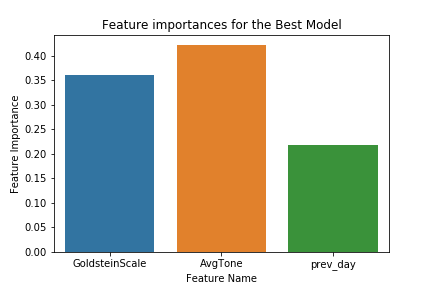
\includegraphics[width=0.8\textwidth]{images/feature_importance.png}
	\caption{The Feature Importances of the Features in the best model}
	\label{fig:featimport}
\end{figure}


Comparing the reference model to the exponentially lagged Random Forests Model on May-June Dow Jones data, The reference model was 50\% accurate, and the exponentially smoothed random forest achieved an accuracy of 62.5\%, which would appear to suggest that the Average Tone and Goldstein Scale values do provide value in terms of predicting shift. 

The predictions are shown in figure \ref{fig:modelpred}, where the magnitude of the differences has been plotted, alongside whether the best model was correct in predicting a positive or negative shift (blanks are weekends or days when the stock market did not operate). There does not appear to be a time based prediction component, the model is just as likely to predict correctly or incorrectly regardless of the time that it is predicting on. The model does not appear to be very good at predicting for large stretches correctly, it correctly predicts for a day or two, and then has incorrect predictions for a similar length of interval. The exception to this is when halfway through the prediction, the model correctly predicts the spike and the subsequent fall and recovery. 

The distribution of magnitude of the positive and negative daily differences is plotted in Figure \ref{fig:distmodel}.  It is apparent that the model is better at predicting smaller differences in the stock market. the majority of incorrect predictions come from larger negative values closer to -500 points and slightly from the positive jumps. There are significantly fewer incorrect predictions when the market jumps between -250 and +250 points. Interestingly, there is a small bump at a large positive value of +1000, suggesting the model was good at predicting large positive values. 

\begin{figure}[H]
	\centering
	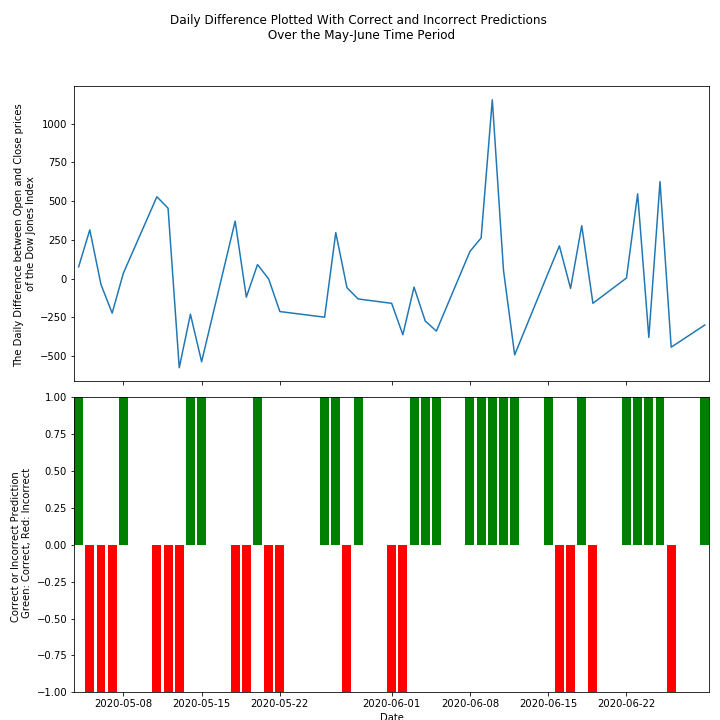
\includegraphics[width=0.8\textwidth]{images/model_pred_time.png}
	\caption{The Dow Jones daily changes in prediction dataset, and whether the model predicted the result correctly or not on a daily basis over the prediction interval of May and June 2020}
	\label{fig:modelpred}
\end{figure}


\begin{figure}[H]
	\centering
	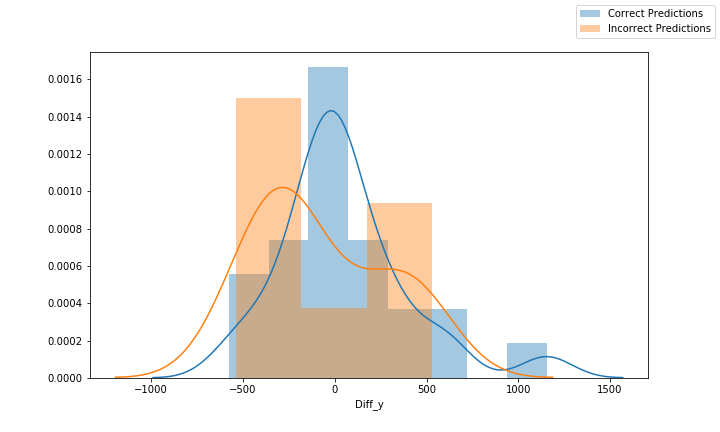
\includegraphics[width=0.8\textwidth]{images/dist_of_model.png}
	\caption{The distribution of the daily differences between open and close prices where the model predicted correctly vs predicted incorrectly}
	\label{fig:distmodel}
\end{figure}

\subsubsection{Portfolio Results}
3 different portfolio styles were tried, firstly a balanced strategy, where half of the capital is used every time shares are bought, and half of the shares are sold whenever shares are sold. This is shown in Figure \ref{fig:port_1}. The second strategy focused on maximising capital, so only \unboldmath$\frac{1}{5}$ of capital was used to buy shares, and $\frac{4}{5}$ of shares were sold whenever shares were sold. This is shown in Figure \ref{fig:port_2}. The final strategy was a shares maximising strategy where $\frac{4}{5}$ of capital was used to buy shares any time shares were brought, and $\frac{1}{5}$ of shares were sold whenever shares were sold. This is shown in Figure \ref{fig:port_3}. All of these strategies started off with no initial shares, and an initial capital of 2000, and used a prediction sensitivity threshold of 60\%. A low threshold was used to maximise the number of decisions the predictive model was taking. Though, this would increase the risk as the model may not be as confident in the prediction. 

\begin{figure}[H]
	\centering
	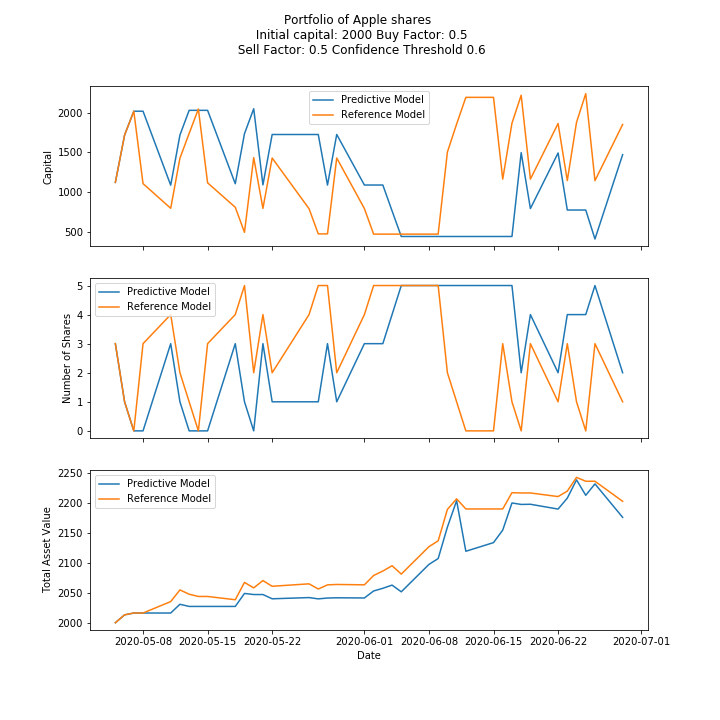
\includegraphics[width=0.65\textwidth]{images/portfolio_1.png}
	\caption{The amount of shares, capital, and Total Asset Value plotted through the time for the first portfolio strategy}
	\label{fig:port_1}
\end{figure}

\begin{figure}[H]
	\centering
	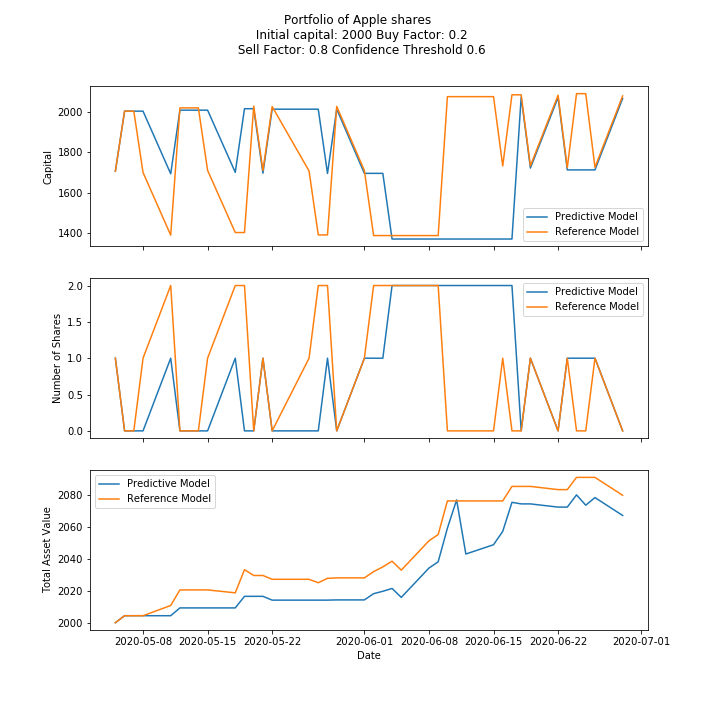
\includegraphics[width=0.65\textwidth]{images/portfolio_2.png}
	\caption{The amount of shares, capital, and Total Asset Value plotted through the time for the second portfolio strategy}
	\label{fig:port_2}
\end{figure}

\begin{figure}[H]
	\centering
	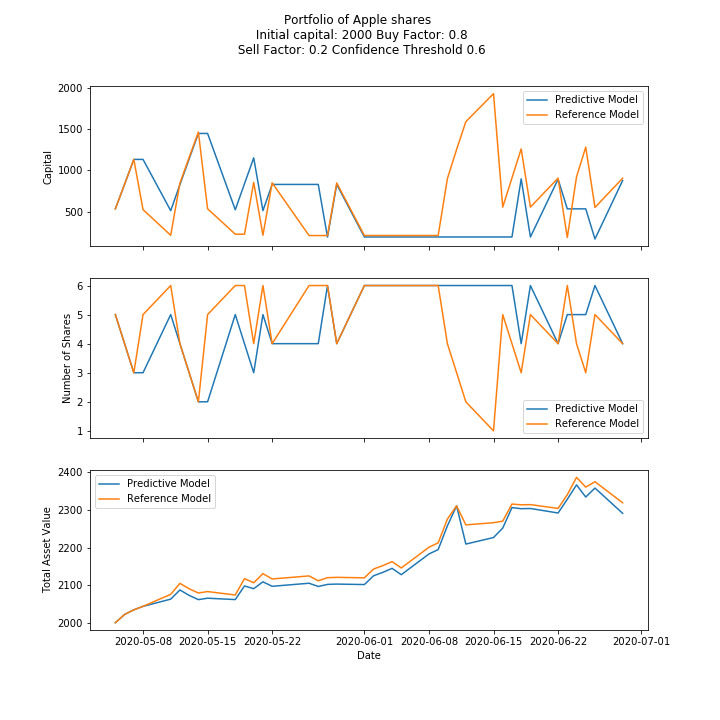
\includegraphics[width=0.65\textwidth]{images/portfolio_3.png}
	\caption{The amount of shares, capital, and Total Asset Value plotted through the time for the third portfolio strategy}
	\label{fig:port_3}
\end{figure}

The first thing to be noted in all of the strategies, is that in all cases, the predictive model was slightly worse over the time period compared to the reference model. This is mostly likely because the predictive model in all cases held on to the stock around the 10th of June, after which the value of the stock decreased considerably and the model was not able to make up the difference within the remaining time period. 

The second point to be made is that all of the strategies accrued financial gain, though the model to maximise shares had the highest total asset value at the end of the time period, followed by the half and half strategy, followed by the capital strategy. The shares total asset value at the end was significantly beyond 2200, which represents more than a 10\% gain in the market over the initial capital investment. However, by comparison the maximising capital strategy only achieved an asset value of 2060, which is a significantly lower growth. The half capital and half shares strategy was doing well, especially recovering after the drop in the middle of the month, but it fell slightly to record a value of nearly 2200, which still is nearly a 10\% gain. However, it should be noted, that for every strategy bar the capital maximising strategy, the majority of the total asset value is represented in stock value and not capital.

